\documentclass{sig-alternate-05-2015}
\usepackage{xspace}

\begin{document}

\setcopyright{acmcopyright}

\conferenceinfo{FSE '16}{November 13--19, 2016, Seattle, WA, USA}




\title{A Doomsday Vault of Software Engineering Tools}
\subtitle{Archiving Software Engineering Tools from ICSE and FSE 2011 through 2014}

\numberofauthors{75}

\author{
\alignauthor
Emerson Murphy-Hill\\
       \affaddr{Department of Computer Science}\\
       \affaddr{NC State University}\\
       \affaddr{Raleigh, NC, USA 27695}\\
       \email{emerson@csc.ncsu.edu}}

\additionalauthors{Additional authors: 
%Example:
% John Smith (The Th{\o}rv{\"a}ld Group,
% email: {\texttt{jsmith@affiliation.org}}) and Julius P.~Kumquat
% (The Kumquat Consortium, email: {\texttt{jpkumquat@consortium.net}}).
%Alphabetical:
Shabbir Abdul (\url{sabdul@ncsu.edu}), 
Varun Aettapu (\url{vaettap@ncsu.edu}), 
Sumeet Agarwal (\url{sagarwa6@ncsu.edu}), 
Sindhu Anangur Vairavel (\url{sanangu@ncsu.edu}), 
Rishi Avinash Anne (\url{raanne@ncsu.edu}), 
Haris Mahmood Ansari (\url{hmansari@ncsu.edu}), 
Ankit Bhandari (\url{abhanda3@ncsu.edu}), 
Anand Bhanu (\url{bhanua@ncsu.edu}), 
Aditya Vinayak Bhise (\url{avbhise@ncsu.edu}), 
Saikrishna Teja Bobba (\url{sbobba3@ncsu.edu}), 
Vineela Boddula (\url{vboddul@ncsu.edu}), 
Venkata Krishna Sailesh Bommisetti (\url{vbommis@ncsu.edu}), 
Dwayne Christian (Chris) Brown (\url{dcbrow10@ncsu.edu}), 
Peter Morgan Chen (\url{pmchen@ncsu.edu}), 
Yi Chun (\url{Yi-Chun}) Chen (\url{ychen74@ncsu.edu}), 
Nikhil Chinthapallee (\url{nchinth@ncsu.edu}), 
Karan Singh Dagar (\url{kdagar@ncsu.edu}), 
Joseph Decker (\url{jdecker@ncsu.edu}), 
Pankti Rakeshkumar Desai (\url{prdesai2@ncsu.edu}), 
Jayant Dhawan (\url{jdhawan2@ncsu.edu}), 
Yihuan Dong (\url{ydong2@ncsu.edu}),
Sarah Elizabeth Elder (\url{seelder@ncsu.edu}), 
Shrenuj Gunvant Gandhi (\url{sgandhi4@ncsu.edu}), 
Jennifer Michelle Green (\url{jmgree17@ncsu.edu}), 
Mohammed Hasibul Hassan (\url{mhhassan@ncsu.edu}), 
Satish Inampudi (\url{sinampu@ncsu.edu}), 
Pragyan Paramita Jena (\url{ppjena@ncsu.edu}), 
Bhargav Rahul (\url{Bhargav}) Jhaveri (\url{bjhaver@ncsu.edu}), 
Apoorv Vijay Joshi (\url{avjoshi@ncsu.edu}), 
Nikhil Josyabhatla (\url{njosyab@ncsu.edu}), 
Sujith Katakam (\url{skataka@ncsu.edu}), 
Juzer Husainy Khambaty (\url{jhkhamba@ncsu.edu}), 
Aneesh Arvind Kher (\url{aakher@ncsu.edu}), 
Craig Kimpel (\url{ckimpal@ncsu.edu}), 
Siddhartha Kollipara (\url{skollip@ncsu.edu}), 
Asish Prabhakar Kottala (\url{akottal@ncsu.edu}), 
Abishek Kumar (\url{akumar21@ncsu.edu}), 
Harini Reddy Kumbum (\url{hkumbum@ncsu.edu}), 
Nitish Pradeep Limaye (\url{nplimaye@ncsu.edu}), 
Apoorv Mahajan (\url{amahaja3@ncsu.edu}), 
Sai Sindhur Malleni (\url{smallen3@ncsu.edu}), 
Sudha Manchukonda (\url{smanchu@ncsu.edu}), 
Kavit Maral Mehta (\url{kmmehta@ncsu.edu}), 
Justin Alan Middleton (\url{jamiddl2@ncsu.edu}), 
Ramakant Moka (\url{rmoka@ncsu.edu}), 
Eesha Gopalakrishna Mulky (\url{egmulky@ncsu.edu}), 
Gauri Naik (\url{gnaik2@ncsu.edu}), 
Shraddha Anil Naik (\url{sanaik2@ncsu.edu}), 
Yashwanth Nallabothu (\url{ynallab@ncsu.edu}), 
Yogesh Nandakumar (\url{ynandak@ncsu.edu}), 
Kairav Sai Padarthy (\url{kspadart@ncsu.edu}), 
Pulkesh Kumar Yadav Pannalal (\url{ppannal@ncsu.edu}), 
Sattwik Pati (\url{spati2@ncsu.edu}), 
Kahan Prabhu (\url{kprabhu@ncsu.edu}), 
Shashank Goud Pulimamidi (\url{spulima@ncsu.edu}), 
Gargi Sandeep Rajadhyaksha (\url{gsrajadh@ncsu.edu}), 
Priyadarshini Rajagopal (\url{prajago4@ncsu.edu}), 
Venkatesh Sambandamoorthy (\url{vsamban@ncsu.edu}), 
Mohan Sammeta (\url{msammet@ncsu.edu}), 
Shaown Sarker (\url{ssarker@ncsu.edu}), 
Anshita Sayal (\url{asayal@ncsu.edu}), 
Vrushti Kamleshkumar Shah (\url{vkshah@ncsu.edu}), 
Esha Sharma (\url{esharma2@ncsu.edu}), 
Saurav Shekhar (\url{sshekha3@ncsu.edu}), 
Sarthak Prabhakar Shetty (\url{spshetty@ncsu.edu}), 
Manish Ramashankar Singh (\url{mrsingh@ncsu.edu}), 
Ankush Kumar Singh (\url{asingh21@ncsu.edu}), 
Vinay Kumar Suryadevara (\url{vksuryad@ncsu.edu}), 
Sumit Kumar Tomer (\url{sktomer@ncsu.edu}), 
Akriti Tripathi (\url{atripat4@ncsu.edu}), 
Jennifer Tsan (\url{jtsan@ncsu.edu}), 
Vivekananda Vakkalanka (\url{vvakkal@ncsu.edu}), 
Alexander Valkovsky (\url{avalkov@ncsu.edu}), 
Rishi Kumar Vardhineni (\url{rkvardhi@ncsu.edu}) and
Manav Verma (\url{mverma4@ncsu.edu}).}
%\date{30 July 1999}

\maketitle
\begin{abstract}
Many innovative software engineering tools appear at the field's premier venues, the 
International Software Engineering Conference (ICSE) and the 
Foundations of Software Engineering (FSE).
But what happens to these tools after they were presented?
In this paper, we spend 10,000 hours %update with real number 
trying to obtain, download, use, and repackage 150 %update
tools from ICSE and FSE's tool demonstration tracks.
Our results enumerate the practical and accidental reasons that
software engineering tools fail to work over time,
and provide practical implications for creating lasting tools.
\end{abstract}


%
% The code below should be generated by the tool at
% http://dl.acm.org/ccs.cfm
\begin{CCSXML}
<ccs2012>
<concept>
<concept_id>10002944.10011123.10010912</concept_id>
<concept_desc>General and reference~Empirical studies</concept_desc>
<concept_significance>300</concept_significance>
</concept>
</ccs2012>
\end{CCSXML}

\ccsdesc[300]{General and reference~Empirical studies}

\printccsdesc

\keywords{Software engineering tools; replication}

\section{Introduction}

Sofware engineering research seeks to better
understand software and how it is built and constructed.
While such understanding in isolation can be insightful,
ultimately a substantial amount of such research 
aims to impact the practice of software engineering.
To do so, researchers can create recommendations
for new software engineering practices, can 
create educational techniques and materials, 
and can create tools.

Arguably creating new tools is the most common
way that sofware engineering researchers
attempt to influence practice.
% evidence? would be good to see what the primary contributions are of a recent ICSE or FSE?
Broadly speaking, tools are software that can
help design and build software.
Examples include a tool that helps mobile application
developers choose which devices to target~\cite{prada},
a tool that checks the use of locks in multithreaded programs~\cite{ernst},
and a tool that creates code from natural language text~\cite{desai}.

While papers describe tools in software engineering venues,
there are several reasons why software engineering researchers 
should make the tools themselves available.
First, the full details of how the tool works, both in terms of its internals
and from an end-user perspective, may not be clear from the paper.
Second, making the tools available can help pracitioners try and adopt
the tools in their work.
Third, it helps facilitate reproducibility by enabling future researchers
to perform studies with the original tools.
Finally, it helps the advancement of the field by allowing others to build on 
existing tools, rather than re-buiding them from scratch.

Despite the benefits of making tools available, in this paper
we catalog the practical difficulties in doing so.
We describe a study that examined the tools presented at the 
premier venues for software engineering research over the 
past several years.
As part of a graduate university course on software engineering, 
we spent 10,000 hours trying to obtain, download, use
and repackage tools from the International Conference
on Sofware Engineering (ICSE) and the Symposium on the Foundations
of Software Engineering (FSE).
In doing so, we make the following three main 
contributions in this paper:

\begin{itemize}
  \item A study that evaluates the difficulty in getting tools 
  		working across a variety of software engineering research.
  \item A synergistic course project for graduate software engineering students 
		that gives students meaningful educational value \emph{and}
		provides the research community value.
  \item XXX existing tools repackaged in automatically-built virtual machines
  		to make it easier for others to use these tools.
\end{itemize}

\section{Related Work}

timeliness

General scientific interest in reproducibility.
How it fits with other Rs.
State of practice.

Software reproducibility outside SE.
Systems~\cite{collberg2016repeatability,proebsting2015repeatability}

Others~\cite{kovacevic2007encourage,vandewalle2009reproducible,stodden2009enabling,klein2012run}.


Arguably as SE researchers we should be the best!

Other fields:
- Data science (doing better - http://zenodo.org)
- MPC journal requires code submission (tarball)
- In general, Math not doing a lot with code sub submissions
- Security, should be able to do VM, but don't (but see Will's paper)
- HPC doesn't (and maybe can't)
- RTC is starting to do it, but maybe shouldn't

`` We argue that, with some exceptions, anything less than the release of source programs is intolerable for results that depend on computation.''~\cite{ince2012case}.

Constant worry is protecting IP in security and HPC

Repeatability in AI-SE: ``depends on who does it''
Reproducibility assessment for 2 papers, plus reproducibility overview~\cite{gonzalez2012reproducibility}


While no studies of software reproducibility in our field,
practical interest.

Artifact evaluation committees. (SIGPLAN, where else?)


\section{Research Questions}

Henceforth, we will simply say \textit{tool}
to refer to software engineering tools presented at
the International Conference on Software Engineering
or Foundations of Software Engineering in their
respective tool demonstration tracks.

\begin{enumerate}
  \item How much effort is required to get tools to work?
  \item What are the barriers to get tools to work?
  \item How much effort is required to get tools to work in virtual machines?
  \item What are the barriers to get tools to work in virtual machines?
  \item To what extent is this study practical to implement in a classroom context?
\end{enumerate}

\section{Course Description}

We conducted the study described in this paper as 
part of a graduate software engineering course
in the Computer Science department at 
North Carolina State University.
The department has about 200 PhD students and 450
MS students in its graduate program.
While graduate students are not required to
take the course, it is one of seven core systems
courses, from which students must take one course.
The department does have a specialty MS degree
track in software 
engineering,\footnote{\url{https://www.csc.ncsu.edu/academics/graduate/degrees/se.php}}
which does require this course.

Course content covers software engineering processes,
software architecture, design patterns, software security,
verification and validation, estimation, project managment,
requirements, certification, and formal 
methods.\footnote{Syllabus: \url{TODO}}
Apart from the course content, involving lectures and
a final exam, the other
major component of the course is the project.
Next, we describe the project for this course 
in prior offerings of the course (Section~\ref{sec:priorProj})
and in the offering described in this paper (Section~\ref{sec:thisProj}).

\subsection{Prior Course Project and Criticism}

%TODO experience report, rather than study? action research?

In prior offerings of the course,
students were essentially given two project offerings.
In one version, students could create
a software engineering tool, such as a plugin for Eclipse.
In the other version, students chose several existing,
similar software engineering tools, and applied them
to open source software, then reflected 
on what they learned about the tools and the 
projects.
Most students opted for the second version.
In both cases, students were required to write up their results.
This project is similar to a course project
assigned by David Notkin at the 
University of Washington.\footnote{\url{https://courses.cs.washington.edu/courses/cse503/}}

After offering this project to students for 
several years, the instructor recognized several
problems the way he had executed it:

\begin{itemize}  
  \item The course did not have enough time to teach students
  		technical writing skills, and thus final papers were 
  		of poor quality, on average. Moreover, while technical
  		communication is a course objective, other types of
  		communication would likely be more valuable to most
  		students, who are non-thesis and industry-focused.   		 
  \item Students had limited exposure to state-of-the-art
  		tools; the tools they chose to study were typically
  		quite basic.
  \item Students appeared to rarely gain technical skills 
  		during the project.  
  \item Most students were not doing \emph{novel} work; each semester,
  		different students wrote similar reports on similar tools,
  		which had no value beyond their educational value. 
\end{itemize}

While the last point may seem odd -- why would a course project need
value beyond its educational value? -- it's not unusual for 
some software enginering courses to have added value,
such as contributing to open source projects~\cite{pedroni2007open,meneely2008rose}.
In the case of the present course, the instructor thought 
that such system development would not be useful to most students
in the course, who typically come in with 1 to 2 years of 
industrial software engineering experience. 

\subsection{New Course Project}

In Fall of 2015, the instructor changed the course project
to allieviate the problems described in the last subsection.
In short, student teams were assigned tools described in a 
a prior research paper at ICSE or FSE, the premier 
venues for software engineering research.
Students were required to obtain the tools, get them running,
and redistribut them.

The instructor chose tool demonstration papers, rather than
full techncial papers, for practical reasons.
Full technical papers may not present a tool; for 
instance, a purely qualitative study that reports on 
empirical findings may have no software to go along with it.
In contrast, tool demo papers almost certainly had a working
tool when the paper was presented at a conference. 

There were several learning goals of the course project:

\begin{itemize}
  \item Gain deep experience with several state-of-the-art
  		software enginering tools, and broad overview of many others;
  \item Effectively read research papers;
  \item How to build virtual machines that contain custom
  		software;
  \item How to script virtual machine creation; and
  \item Oral communication skills. 
\end{itemize}

In the remainder of this section, we describe project
activities, requirements, and deliverables.

\subsubsection{Team Formation and Tool Selection}

The instructor formed teams of about 5 students by randomly
selecting about 4 on-campus students and possibly 1 off-campus, distance
education student.

During class, the instructor asked teams to find the ICSE
and FSE demonstration tracks online, skim the papers from those
tracks, and extract several pieces of information:
the venue, the paper name, the tool name, any links to source
code or binaries for the tools, the technologies involved in the 
tool's creation, and a rough estimate of how 
difficult the team thought it would be to get the tool working.
Teams put this information on a shared spreadsheet with one row per paper.
We collected papers from from 2014, the most recent year either ICSE or FSE
papers will officially posted online, to 2009.
In total, we collected 188 papers from 12 conferences.

Teams were then given the opportunity to look over the list of
tools, and identify tools they might want to work on.
During the following class period, teams chose N tools to work on,
where N was the number of people on the team.
Each tool could be assigned to one and only one tool.

Because some tools were in high demand and some in low demand, for fairness,
teams chose tools in a round-robin draft,
that is, one team chose a tool, then the next team chose a tool, and so on,
until all teams had chosen one tool, and then the first team chooses a second
tool, and the next team chooses a second tool, and so on.
At the time of the draft, 100 students in the class, so the tools eligible
for selection were the 100 most recent tools, which included all tools
from 2012--2014, and a few from 2011.

\subsubsection{Obtaining Tools}

After teams were assigned tools, their first task was to 
obtain the tools, including the source code, if possible,
and the binary if not.
For tools that were deployed (or partially deployed) via a web service, 
students were required to obtain the source or binary for
the service as well; in short, the students needed to
obtain all software components necessary to run the tool
in isolation. 

Teams were instructed to first try to 
obtain the tool from links in the paper itself or via
the web.
If teams could not find the tool, the teams
were instructed to ask the authors, using an email
template show in Figure~\ref{fig:email}.
To minimize communication with the authors, 
the email contained requests for several author
piece of information, the need for which will become 
clear later in this section.
Students were instructed to customize this template,
but to use it as a starting point. 
Full instructions for use of this template can be found 
online.\footnote{\url{https://docs.google.com/document/d/1dWvHS8gf37MgYafqOSl3BJzHYkdG1BHgDT4CYe_QN1I/edit?usp=sharing}}
Teams were asked to include the instructor in
all communications with authors.

\begin{figure}[t]

\noindent
To: <AUTHORS OF PAPER, BUT NOT MORE THAN THE FIRST 5 AUTHORS>

\noindent
Subject: Regarding your tool, <TOOLNAME>

\noindent
Dear Dr. <LASTNAME> and colleagues,

I enjoyed reading your paper <PAPER TITLE>. As part of a graduate software engineering 
class at NC State University, my team has chosen to use the tool <TOOLNAME> as part of our 
class project. In short, the class is using tools from the past few ICSEs and FSEs, then putting 
all those tools in an accessible form (e.g., virtual machine) in central location. Our project is 
supervised by Dr. Emerson Murphy-Hill (CC'd via ncsu-csc-510\@googlegroups.com). When our 
project is complete, we plan on aggregating our results (e.g., how many tools could we get 
working, how easy was it, etc) into a research paper.

Because my grade rests on your tool, I am motivated to get it working. I have a few questions 
for you before I get started.

May I have permission to redistribute an executable version of your tool? Specifically, we plan 
on putting your tool in a virtual machine, then posting that VM on the public internet.

May I have permission to redistribute the source code for your tool? Specifically, I plan on 
getting the tool building into the virtual machine (by way of Vagrant) and posting the build scripts 
on GitHub.

Could you please send me a link (or attachment) to the executable version of your tool? I have 
attempted to find the tool on the internet, but have been unsuccessful.

Could you please send me a link (or attachment) to the source code of your tool? I have 
attempted to find it on the internet, but have been unsuccessful.

I've had some trouble getting the tool to work... <describe what you tried, describe what you 
expected to happen, describe what actually happened.>

Thank you very much,

<YOUR NAME>

\caption{An email template used by students for obtaining tools.}\label{fig:email}

\end{figure}

%TODO how long did we give authors to provide the tools? 10 days? 7 days?

\subsubsection{Getting the Tools Working}

Once students had obtained the tools, they had two weeks to get 
the tools working.
Because some tools may only work in the very specific situations 
described in their papers,
teams were required to get the tools ``working'' as it was described
in the paper.
Teams were allowed to use any means necessary to get the tools working,
including asking classmates for help, but were discouraged from
harassing the tools' authors.
At the end of the two weeks, if the tool was obtained and working,
teams certified that the tool as working on the spreadsheet.

If a team could not get a tool working for whatever reason, 
several things happened.
First, the team must certify the tool as ``unworkable.''
Second, the team would be assigned a new tool by moving down the list
of tools, and the process would start again.
Third, the tool certified as ``unworkable'' would be made available 
to the other teams to try to get working.

The instructor created a disincentive for students to unnecessariyl 
certify a tool as unworkable.
If a team got an unworkable tool working, the team that certified it as  
unworkable had their final course grade reduced by a minor 
grade (for example, from an A to an A- or from a C to a C-).
The team that gets the ``unworkable" tool working gets their final grade increased
by a minor grade point.
Furthermore, the only way to get an A+ course is to be on a team
that gets an unworkable tool working.

\subsubsection{Getting the Tools Working in a Virtual Machine}

The first graded deliverable was a VirtualBox virtual machine
image that contained an operating system, the tool, any
and other software required by the tool (such as Eclipse),
documentation, and license information.
The goal of creating this image was to make it as
easy as possible for future potential users to try
the tool out; in essence, any ``fiddling'' required to get
a tool working would not have to be done by the user.
%VirtualBox is free and open source, and can be run on Windows,
%Linux, OS X, or Solaris.

The grading rubric for the image\footnote{\url{https://docs.google.com/spreadsheets/d/1zGwF_TbGCmrwH1vqY2_OHAQg7umd4zyAepHiirdb-yM/edit?usp=sharing}}
additionally specified that minimal work is required
on the part of the user to see the tool in action,
that the technology stack does not contain any proprietary 
software that is not not stricly necessary,
and that the image is as small as possible.

% there was a second VM submission

\subsubsection{Building the Virtual Machine Image Automatically}

After building a basic virtual machine image by hand,
teams next built Vagrant scripts that built virtual machines
automatically.
The main goal of creating the script was to add 
transparency to the process
of installing the tool; if future users want to install the tool
in their own development environment, the script provides a
specification for doing so.

The grading rubric for the virtual machine 
script\footnote{\url{https://docs.google.com/spreadsheets/d/1qSt63AjwyiCRHCU-MMoTSDx_qPuWn7U4_QmjwC_Ghds/edit?usp=sharing}}
was largely the same as for the hand-built image.
For instance, some things that were easy to do in a hand-built 
image turned out difficult in the script, such as changing 
the username and password, so such requirements were 
not included in the grading rubric for the script.
The most substantial additional requirement for the script
was that it uses ``standard and stable external resources 
whenever possible (e.g., www.vagrantbox.es, rather than a 
hand-built box)''.

\subsubsection{Redistributing the Tools}

Teams were required to establish GitHub repositories 
for each tool that their team was assigned -- working or not.
The main goal was to share the work the teams had 
done with others.
We created an organization to house each repository,
which can be found 
online.\footnote{\url{https://github.com/SoftwareEngineeringToolDemos/}}

If the original tool contained a license to redistribute
the source code, or the paper authors gave us explicit
permission to do so, we redistributed that code 
in our tool's repository.
The same applied to the tools' binary.
If the tool was working, 
vagrant scripts were also included in the repository,
regardless of whether we had permission to redistribute
the tool; if we did not, users would have to contact the 
original authors and drop in the tool (a binary, for instance)
for the script to work.
Even if the tool was not available to us, we created
a mostly empty repository, for consistency.

%TODO: for consistency: we, instructor, students, teams -> consistency
%		pref for ``we'': the effort was quite collaborative, with me providing
%		some technical help, students providing input into the process, TAs the same

For tools for which we had source code,
whenever possible teams included the history
of that source code, for completeness.
Ideally, tools that were already hosted
on GitHub could be forked by the team,
maintaining not just history but also an 
explicit connection to the original repository.
When original tool were hosted elsewhere, such
as in subversion on Google Projects, 
teams migrated source code history to GitHub.

Teams added a readme file to each tool's repository
that conveyed some basic information about
the tool, including 
links to the original paper and
original project webpage, 
as well as acknowledgements.
The rubric outlined a number of small,
specific requirements for the readme to
ensure consistency.\footnote{\url{https://docs.google.com/spreadsheets/d/1ufh-XiNFY1jRvehDN_JulYQTRVHzuEDru6stPAyjxdc/edit?usp=sharing}}

When teams had permission to redistribute
the virtual machine image containing the tool,
readmes also contained links to those images.
The images were hosted on the instructor's 
Google Drive account, which provides unlimited
cloud storage.\footnote{\url{https://support.google.com/a/answer/2856827}}
Such large capacity storage is necessary because each
image occupies several gigabytes of space.

\subsubsection{Presenting Tools}

For the communication part of the class,
teams were to present each working tool in front of the class
for a 5 minute demonstration.
The grading rubric specified, among other requirements,
that the presentations explained what problem the 
tool was built to solve, to give a simple enough
example that the tool could be understood,
and to be realistic enough to be 
compelling.\footnote{\url{https://docs.google.com/spreadsheets/d/1Mb8yacxIP233kmjn3J_JtjOfJuIjmSHnMKttr1CVxCM/edit?usp=sharing}}
Teams also prepared a video demo of each working tool,
posted on YouTube and linked to from the virtual machine
image and the GitHub readme.

\subsubsection{Evaluations}

Teams' deliverables were evaluated by their 
peers and by two teachers' assistants (TAs).
While both peers and TAs evaluated the deliverables
for quality and consistency, only the TA evaluations
counted towards teams' grades.

Teams completed peer evaluations of other teams' hand-built 
virtual machines and GitHub repositories.
This entailed reading the original paper to understand
how the tool was supposed to work, 
using the tool in the virtual machine,
and comparing deliverables to the grading rubrics.
When students found defects, they filed issues 
in the repositories issue tracker and provided
fixes for simple defects using pull requests.

%TODO should really link to these, too. can we make Moodle public?

Hand-build virtual machine images were evaluated in 
two rounds by the TAs, where students enahanced their
images between rounds and the rubrics were updated
for the second round based on what the TAs 
observed in the first.
Likewise, vagrant scripts were evaluated in two rounds
by the TAs.
Finally, TAs evaluated all artifacts (images, vagrant 
scripts, and repositories) together in a final project 
evaluation.

\subsubsection{Data Collection and Contributions}

As part of the final project submission, 
the instructor collected data about 
each tool in the form of a survey.
This tool survey asked, for instance, how long
the team estimated they spent on getting 
the tool working.
Teams reported data for all tools, except six tools,
all from a single team.
The team certified six tools as unworkable,
but all students who worked on the tools dropped
the course.
The remaining student was unable 
to provide accurate data about the tools, and thus 
no reports were submitted.

Each student also submitted a second survey that
asked students what they thought about the project,
and whether they wanted to participate as an
author of this paper.
Two students opted not to participate as an author.
Data was also collected from standardized and 
anonymous course evaluation forms, forms
that are used for all courses 
across the university.

This paper was written primarily by the first author,
the instructor of the course, after the course 
had ended.
The paper's source and history can also be found 
on GitHub.\footnote{\url{https://github.com/SoftwareEngineeringToolDemos/paper}}
The technical work was conducted primarily by the students.

\section{Example Tool}

Sketch example tool here, with all the pieces.
It would be nice if it exemplified some issues 
brought up later, such as technology stack licensing.

\section{Procedure}

No cost, but demos ok. (How many did this happen with?)

Tools where tool could convievably be put into a virtual machine. How many didn't fit?

\section{Results}

\newcommand{\durationTotal}{6706\xspace}
\newcommand{\durationCorresponding}{2\xspace}
\newcommand{\durationWorking}{10\xspace}
\newcommand{\durationVM}{10\xspace}
\newcommand{\durationVagrant}{15\xspace}
\newcommand{\durationWorkingOnWorkable}{10\xspace}
\newcommand{\durationWorkingOnUnWorkable}{10\xspace}
\newcommand{\emailsSent}{3\xspace}
\newcommand{\emailsRecieved}{2\xspace}
\newcommand{\durationAuthorResponse}{15\xspace}
\newcommand{\durationAuthorResponseCountHigh}{20\xspace}
\newcommand{\emailsHelpful}{82\%\xspace}
\newcommand{\emailsFriendly}{85\%\xspace}
\newcommand{\emailsIntimidating}{4\%\xspace}
\newcommand{\emailsAnnoyed}{10\%\xspace}
\newcommand{\emailsPercentSent}{92\%\xspace}
\newcommand{\contactOSSed}{2\xspace}
\newcommand{\contactFixLink}{3\xspace}
\newcommand{\contactHosted}{4\xspace}
\newcommand{\contactFixBug}{8\xspace}
\newcommand{\contactFixDepl}{2\xspace}
\newcommand{\papersWithLinks}{62\%\xspace}
\newcommand{\papersWithLinksDead}{7\%\xspace}
\newcommand{\papersWithLinksRevived}{44\%\xspace}
\newcommand{\obtainPaper}{42\%\xspace}
\newcommand{\obtainGoogle}{19\%\xspace}
\newcommand{\obtainEmail}{20\%\xspace}
\newcommand{\obtainNot}{20\%\xspace}
\newcommand{\onlineGitHub}{25\%\xspace}
\newcommand{\onlineSourceforge}{3\%\xspace}
\newcommand{\onlineGcode}{4\%\xspace}
\newcommand{\onlinePersonalSite}{28\%\xspace}
\newcommand{\onlineNotAvail}{39\%\xspace}
\newcommand{\onlineCodeplex}{2\%\xspace}
\newcommand{\onlineBitbucket}{3\%\xspace}
\newcommand{\working}{63\%\xspace}
\newcommand{\unworkPay}{2\xspace}
\newcommand{\unworkInternal}{9\xspace}
\newcommand{\unworkNoResponseToAsk}{13\xspace}
\newcommand{\unworkTooLate}{3\xspace}
\newcommand{\unworkCouldntWorkIt}{19\xspace}
\newcommand{\serviceRunning}{8\xspace}
\newcommand{\serviceRunningLater}{2\xspace}
\newcommand{\serviceRunningNever}{4\xspace}
\newcommand{\redistPermissionArtifact}{43\xspace}
\newcommand{\redistPermissionEmail}{31\xspace}
\newcommand{\licenseMIT}{7\xspace}
\newcommand{\licenseGPL2}{5\xspace}
\newcommand{\licenseApache2}{7\xspace}
\newcommand{\licenseGPL3}{4\xspace}
\newcommand{\licenseBSD2}{6\xspace}
\newcommand{\licenseLGPL21}{2\xspace}
\newcommand{\licenseMPL}{2\xspace}
\newcommand{\licenseEPL}{14\xspace}
\newcommand{\depWindows}{22\xspace}
\newcommand{\depVS}{6\xspace}
\newcommand{\permissionToRedistribute}{49\xspace}



\newcommand{\projectLikeThis}{45\%\xspace}
\newcommand{\projectLikeOther}{26\%\xspace}
\newcommand{\projectDontCare}{30\%\xspace}

\subsection{RQ1 and RQ2}

\subsubsection{Effort}

Through a survey near the end of the course, 
teams estimated how long they spent
corresponding with paper authors,
getting a tool to work,
getting it to work in a virtual machine,
and getting it to work with vagrant.
The median time teams spent corresponding with
authors was \durationCorresponding hours.
For tools where teams obtained the tool,
they spent a median of \durationWorking hours
trying to get it to work.
For tools where the teams got a tool working,
they spent a median of \durationVM getting it working 
in a virtual machine image and
\durationVagrant hours generating a working tool
image with Vagrant.
In total, teams spent \durationTotal hours working
on all tools combined.

%TODO box/vio plot?

The survey also asked participants if they spent
additional time on their projects.
In addition to project requirements like establishing
the GitHub repository, teams 
reported spending additional time 
learning about their tools,
searching for the tool on the web,
waiting for author replies,
obtaining the license for a tool,
figuring out what dependencies a tool had,
obtaining a Solaris base box for Vagrant,
and
getting a tool to work with a variety of examples.

\subsubsection{Interactions with Authors}

\begin{figure}[!ht]
  \centering
    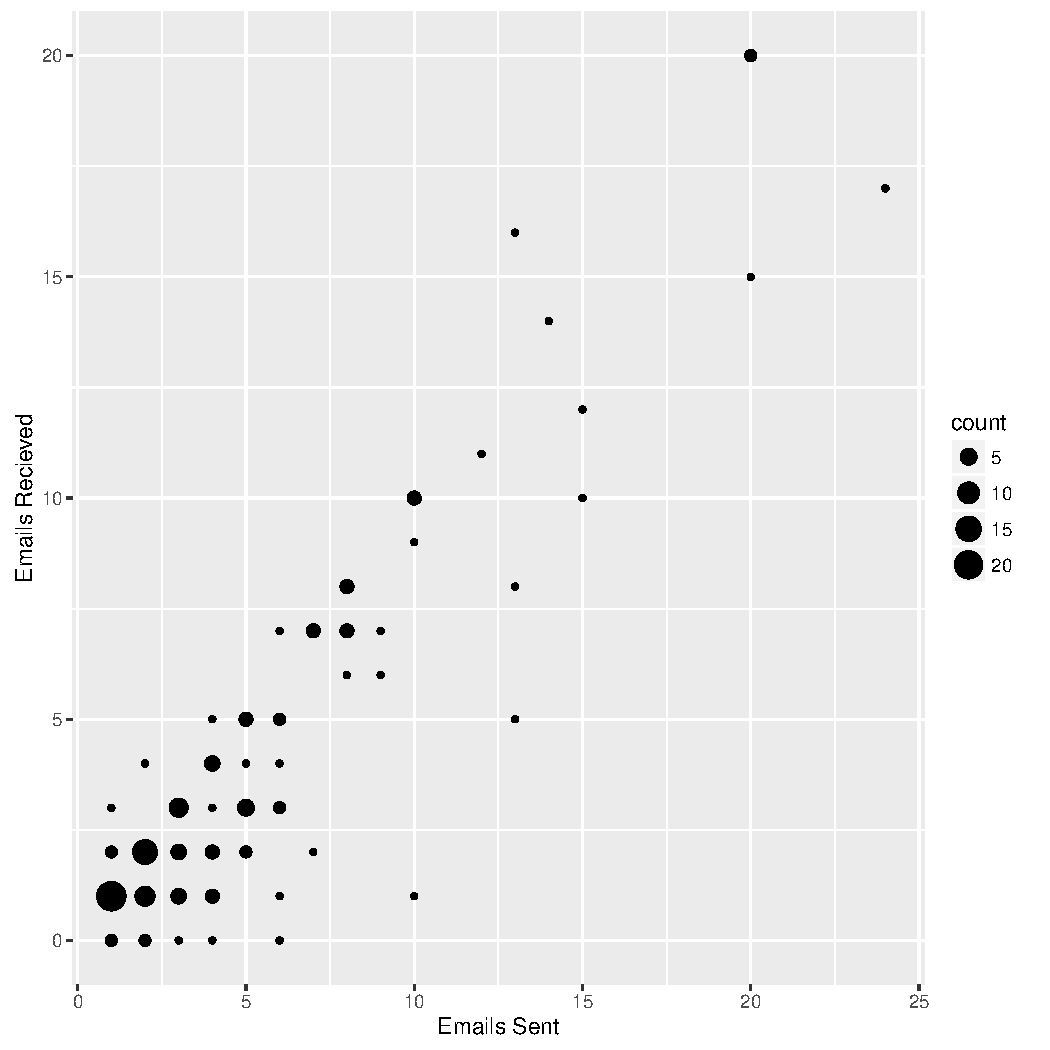
\includegraphics[width=0.5\textwidth]{emailPlot.pdf}
  \caption{Summary of emails sent and received.}\label{fig:emailSnR}
\end{figure}

\begin{figure}[!ht]
  \centering
    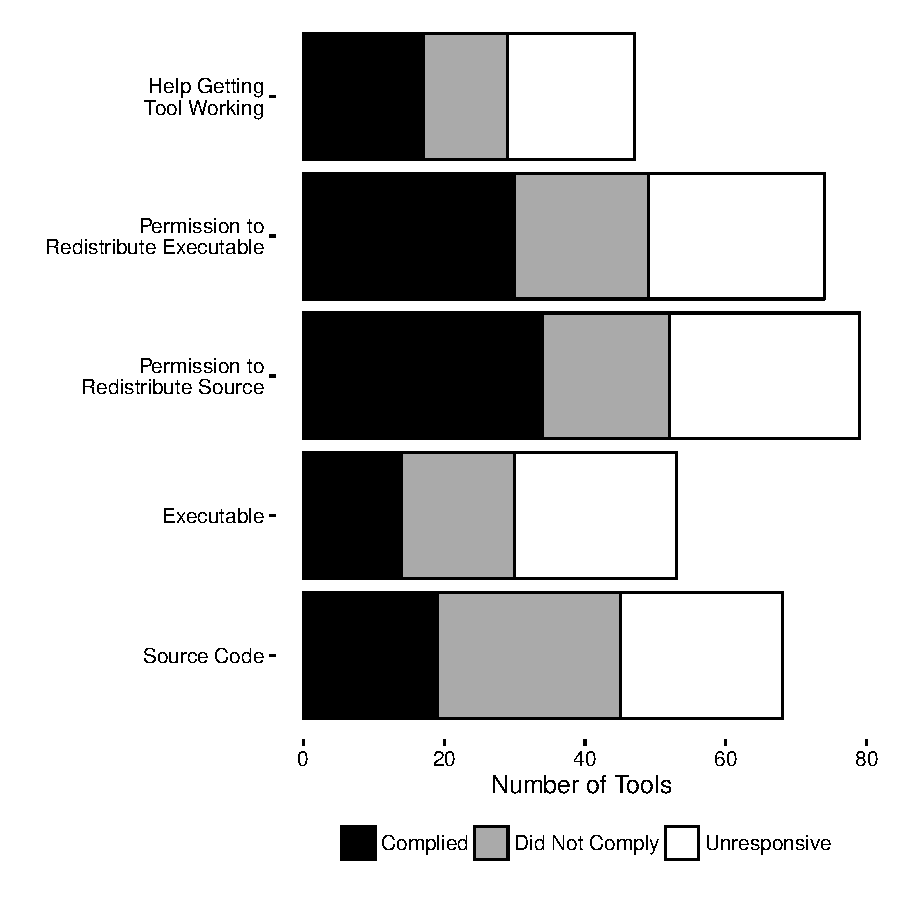
\includegraphics[width=0.5\textwidth]{requestPlot.pdf}
  \caption{Authors compliance with teams' tool requests.}\label{fig:requests}
\end{figure}

Because a significant portion of participants' time was
spent corresponding with the authors,
the survey also asked teams about their email interactions.
Overall, teams sent emails for \emailsPercentSent of tools.
Teams sent a median of \emailsSent and recieved 
a median of \emailsRecieved emails from each author.
Figure~\ref{fig:emailSnR} summarizes the number of emails
we sent and received, where the size of each dot
represents the number of tools that had
that many emails sent and received.
We see that, overall, few emails were required
and authors appeared generally responsive.

While authors were generally responsive to emails,
they were not necessarily responsive or compliant 
with the requests contained in those emails.
Figure~\ref{fig:requests} lists what teams requested from authors
(horizontally) and whether authors complied (colors).
Overall, each kind of request was met with substantial non-response and
non-compliance.
Beyond these requests, teams reported needing to ask for 
license keys and
an old version of a dependency.

%TODO should check to see which projects have licenses, 
%and perhaps students didn't need to send emails

%TODO: binary/executable for consistency throughout paper

We also estimated how much
time authors spent reading and responding to our emails.
To minimize authors' effort, we did not ask authors directly.
Instead, we asked teams to estimate how much time authors spent 
reading and responding to our emails, including time for 
any background work such as restarting servers.
Teams estimated that a median of \durationAuthorResponse minutes 
was spent, with \durationAuthorResponseCountHigh tool authors having
to spend more than an hour.

Teams also reported about the tone of the response they received from 
authors.
Teams felt that \emailsHelpful of responses were helpful and
\emailsFriendly were friendly.
Only \emailsIntimidating felt the responses were intimidating
and \emailsAnnoyed seemed annoyed.

In freeform text on the survey, teams reported whether 
there was anything missing from the tool when they first
got it.
Teams reported missing configuration files
settings that needed to be edited before use, 
information about IDE compatibility,
sample input,
and steps required for installation.                                                                                                               

\subsubsection{Missing Information}

In contacting the authors, authors sometimes made
changes to their tools or supporting infrastructure.
Teams reported that authors fixed bugs in \contactFixBug tools,
started hosting \contactHosted tools on a public repository,
fixed web links to \contactFixLink tool binaries,
added open source licenses to \contactOSSed tools,
and fixed deployment issues for \contactFixDepl tools.
Teams also reported teams fixing problems with dependencies,
fixing other kinds of links, 
modifying an existing readme,
and adding a vagrant script to an existing repository.

Teams found that about \papersWithLinks papers
contained links to online information about their tools.
Team also found that \papersWithLinksDead papers
had links that were no longer functional,
where \papersWithLinksRevived of those links
being fixed after teams emailed the papers' authors.

When it came to obtaining the tools, 42\%
could be obtained from links in 
the papers directly.
\obtainGoogle could not be obtained from
links in the papers themselves, but could be
from searching the web.
When those failed, another \obtainEmail were 
obtained after emailing the authors.
\obtainNot of tools could not be obtained
by teams at all.

We also assessed where the source code for tools are available,
apart from our GitHub repositories.
\onlineNotAvail of tools had no source code available 
on line.
\onlinePersonalSite of tools had source code hosted
on an author's personal website.
Many tools were available on open code repositories:
\onlineGitHub on GitHub, 
\onlineGcode on Google Code,
\onlineSourceforge on Souceforge,
\onlineBitbucket on Bitbucket,
and \onlineCodeplex on CodePlex.

\subsubsection{Getting Tools Working}

In total, teams marked \working tools as working.
The remaing tools were marked ``unworkable'' for a 
several of reasons.
The most common reason teams marked tools as unworkable
was that the teams could not get the tools 
working (\unworkCouldntWorkIt tools),
typically due to build errors or mismatches between
the way the downloaded tool worked and the way 
it was described in the paper.
A common problem for these tools was dependencies on
software whose versions were unspecified 
(and at least once forgotten by the author), and teams
failed to get the tools working with the versions they
tried.
Teams also described having issues with 
tool configuration,
missing functionality, and
missing or corrupted program files or data.

Teams were unable to mark tools as working 
for a variety of other reasons, as well.
For \unworkNoResponseToAsk tools, teams reported asking for a tool,
but recieving no response from the authors.
For \unworkTooLate tools, teams eventually got a response with the tool, 
but it was  too late.
%TODO how late is too late?
\unworkInternal tools were not available outside the organization
they were developed in.
\unworkPay tools had software dependencies on for-pay tools; 
the may have worked if we had been willing to pay 
for the dependencies.

Several tools were not available to us, 
and the authors were unwilling or unable to do so.
For two tools, the author was simply unavailable,
without further explanation.
For one tool, the author was uncomfortable making 
the tool available.
For another, the author said the tool was only a prototype.
For another, the author stated that the tool had too
many dependencies with other tools.
For another, the author stated that the tool does not
exist anymore.

Several of the tools we analyzed were a service or had a
service component; for instance, several tools
ran as web applications on the creator's website.
If the service is running, services provide a convenient way
for users to try a tool.
In total, for \serviceRunning tools, teams 
reported that the service was running when the teams tried
to access it.
For \serviceRunningLater tools, teams reported that the service
was not running, but the authors got the service running
after the teams emailed them.
For \serviceRunningNever tools, teams reported that the service
never worked when they tried it.  

\subsubsection{Licensing and Permissions}

\redistPermissionArtifact tools were open-sourced, 
under a variety of licenses.
Common licenses were:
\licenseEPL had an Eclipse Public License license,
\licenseMIT had an MIT license,
\licenseApache2 had an Apache 2.0 license,
\licenseBSD2 has a BSD 2.0 license,
\licenseGPL2 had a GPL 2.0 license,
\licenseGPL3 had a GPL 3.0 license,
\licenseLGPL21 has a LGPL 2.0 license,
\licenseMPL has a Microsoft Public License.
Although they did not have an explicit license,
authors of \redistPermissionEmail tools granted us
permission to redistribute via email.
Two tools were freely available online
with an open source license, but the authors of those
tools specifically asked us \emph{not} to redistribute the
tool; although we honored the authors' requests,
the requests nonetheless directly conflicts
with those tools' licenses.  

Our ability to redistribute virtual machines of the tools were
further restricted by the tools' dependencies.
The most common dependencies were on the Windows 
operating system (\depWindows tools).
\depVS tools were dependent on Visual Studio.
A few other tools depended on other commercial 
operating systems and tools.
 
After excluding tools 
that we did not get working,
that we did not have permission to redistribute, and 
that relied on software we did not have permission to redistribute,
\permissionToRedistribute tools remained.
We have made these tools publicly available in virtual machines 
images online.\footnote{\url{http://go.ncsu.edu/SE-tool-VMs}}
Our GitHub repositories link to these virtual machine images,
and contain relevant tool artifacts such as source code
and binaries.
A total of 62 repositories 
% based on https://github.com/search?q=org%3ASoftwareEngineeringToolDemos+Vagrant.configure&ref=searchresults&type=Code&utf8=%E2%9C%93
contain vagrant scripts to build 
virtual machines that contain the tools. 


\subsubsection{Challenge: Tool Cannot Be Obtained}

What percent of tool links were dead?
What percent of tools said they were available in the paper, but the tool could not be obtained?
What percent of tools were being planned to be commercialized? What were actually commercial?
What percent of tools could we use if we had paid for them?

\subsubsection{Challenge: Disappearing Tools}

One author said tool just doesn't exist anymore.

Another author had to dig tool out of long term archive.

Several authors (what percent?) has tools hosted on Google code, even though it was dying.
Did we save 'em?

\subsubsection{Challenge: Author non-responsive}

%TODO: look at righthand column for tool; indications of why tools not working?

\subsubsection{Challenge: Technical Difficulties}

\subsubsection{Challenge: Inconsistencies}

One tool required to different VMs because two features needed different prereqs.

Some tools versioned differently.

\subsection{RQ3 and RQ4}


\subsection{Course Results}

Viewed in the context of a university course,
students viewed the course project negatively,
based on two main metrics.
First, many students dropped the course; 
at its peak, the course was full and had a full
waiting list with a combined 105 students.
By the end of the course, only 58 students remained.
%based on mypack, minus one student marked as `Crs Wdraw'
Second, the university-administered evaluations for
the course and course project were low.
All quantitative metrics for the course were below
the Computer Science department average, and were
lower than for courses the instructor has previously
taught.
Specifically, the most common response to the question
of whether the course project was a valuable aid to learning
was ``strongly disagree''.
What accounts for this negative reaction?

With respect to students dropping the course, students were asked
in the non-anonymous survey at the end of the course whether they knew
students who dropped, and if so, whether they knew why.
While students cited some external reasons, the 
primary one appeared to be that the course was more work
than they had expected.
Although other changes had been made to the course, 
most notably ``flipping'' the lectures~\cite{flipped},
the main one was the project, so the project load
was likely responsible for the drops.

With respect to low student evaluations of the project,
the problem appears to be with several aspects of project
design, rather than a fundamental issue with the project itself.
In the non-anonymous survey, students were given a brief description
of the old project, and were asked which version of the course project
they would prefer.
\projectLikeThis of students preferred the present course project,
\projectLikeOther would prefer the past course project,
and the remaining students had no preference.
Nonetheless, several areas of the course project were challenging,
as described below.

\textbf{Lack of Teamwork.}
  	Teamwork was critical to a successful project, because a single student
  	is unlikely to have all the technical skills necessary to get an
  	arbitrary tool working.
  	While the instructor explaind this to students early on, 
  	he did not provide an environment that was conducive to teamwork.
  	First, no specific collaboration technologies or practices were encouraged,
  	such as Slack, scrum, or cloud-based virtual machines.
  	Second, the easiest way to break down work was to assign one person in a team
  	to work on one tool; because each tool generally worked independently
  	from other tools, it appeared that teammates worked in a fairly siloed way.  	
  	Third, teams lacked cohesiveness because teammates were assigned randomly.
  	Because many students dropped the course, team cohesiveness may have 
	been reduced further.
	Teamwork problems can likely be improved substantially in the future by 
	educating students on and providing collaboration technologies, and allowing
	teams to choose their own members. 

\textbf{Uneven Tool Difficulties.}
  	Some tools are simple, others are complex; likewise,
  	some tools were easy to get working, while others were extremely difficult.
  	The instructor originally aimed to improve fairness by assigning multiple tools
  	to teams, so that average tool difficulty across teams should be roughly equivalent.
  	However, the siloing within teams still meant that some students were doing
  	significantly more work than other students.  
  	Breaking down the silos may improve this inequity problem.
  	This may also be an opportunity to create an assignment that applies the course
  	material on effort and risk estimation.   	

\textbf{Vagrant Scripting.}
  	Vagrant scripting turned out more challenging than anticipated.
  	One reason was that install software on Windows machines is difficult
  	due to operating system security checks.
  	Another difficulty was some scripts needed large files, which GitHub could not
  	store, so these scripts needed to load data from other locations 
  	(such as Google Drive), decreasing the likelihood that these scripts will
  	continue to function correctly over time. 
  	Building vagrant vagrant scripts should be easier in the future, now that
  	we have a repository of examples that include, for instance, how to
  	use a Windows package manager and how to 
  	install Eclipse and load Eclipse workspaces. 
  	One way to approach quality problems is by treating them as testing and 
  	continuous integration problems; Travis CI,
  	for instance, may be appropriate for building VMs automatically,
  	assessing the quality of those VMs with test automation,
  	and making public the VMs and Travis scripts.

\textbf{Unusual Grading.} 
	The instructor recognized that the grading strategy of making substantial
	grade adjustments when teams got unworkable tools working would be 
	controversial among students.
	Four out of 44 students complained about this in the anonymous course
	evaluation.
	Only one team ended up getting an unworkable tool working, and this team expressed
	some hesitation in doing so because it meant a negative repercussions for their
	classmates.
	Nonetheless, in the opinion of the instructor, the grading strategy was effective
	in making sure teams tried sufficiently hard to get their tools working. 
 	Future iterations of the project may explore alternate grading options.

\textbf{In-Class Presentations.}
  	Although in-class presentations were only 5 minutes per tool, as a whole they
  	took up an inordinate amount of class time.
  	For future iterations of the projects, students will instead make videos posted
  	online about their tools, and perhaps only one tool per team will be presented
  	in class.
 
Finally, despite the challenges with the course, the instructor's opinion is that 
the course was highly worthwhile.
He knows of no other software enginering courses that integrate research into 
teaching to the degree that this one does, while at the same time capitalizing
on the existing talents of computer science graduate students for the greater 
good.
While educational outcomes can be strengthened by deeper integration of the lecture
material into project work, as a whole, the instructor believes that 
the project was an improvement over the prior project.
On the other hand, the project was so radically different from prior 
projects -- perhaps to a mutinous degree -- that trying it is a risky 
proposition for untenured instructors.

\subsubsection{Challenge: Tool Licensing}

University grey area.

\subsubsection{Challenge: Technology Stack Licensing}

\subsubsection{Challenge: Author Doesn't Want Redistribution}

Even when tool is available

\section{Conclusions}

Some other things.

%ACKNOWLEDGMENTS are optional
%\section{Acknowledgments}


\bibliographystyle{abbrv}
\bibliography{references}

\end{document}
